\documentclass{handout}

% \SetInstructor{Lt Col James Phillips}
\SetCourseTitle{ECE231: Electrical Circuits and Systems I}
\SetSemester{Block II}
\SetHandoutTitle{Lecture 16: Operational Amplifiers - Part 3: Circuit Design}

%\SetDueDate{1 Jan 2016}
%\ShowAllBlanks

\showsoln \setsolncolor{red}

\begin{document}
\maketitle

\textbf{OBJECTIVES:}
\begin{enumerate}
\item Understand how to cascade Op Amps to design more complex circuits
\end{enumerate}

\textbf{READING}
\begin{description}
\item [Required]:
\begin{itemize}
\item  Textbook, section 4.5, pages 201--208
\end{itemize}
\item [Optional]: None
\end{description}

\section{Review of our Op Amp {\em Building Blocks}}
In this section, I will offer a quick review of our four Op Amp building block circuits plus one new one:
\begin{enumerate}
\item Non-inverting Amplifier
\item Inverting Amplifier
\item Inverting Summer
\item Differential Amplifier or Subtractor
\item Buffer
\end{enumerate}

This list is not all inclusive.

In addition, I will show figures with the Op Amps inputs connected to thevenin circuits.  These circuits can represent non-ideal sources (with internal resistances) or any resistive circuit.  This will allow us to further explore the concept of loading at the input terminals.

\newpage
\clearpage
\pagebreak

\subsection{Non-inverting Amplifier}
Figure \ref{fig: NonInvertingAmplifier} shows a non-inverting amplifier connected to a thevenin circuit; as mentioned above, this input circuit can represent a non-ideal source or any other resistive circuit.  Since we know that zero current flows into the input terminals of the Op Amp, we can deduce that there is no input loading that results from $R_T$; that is there is no voltage drop or change to the transfer characteristic.

\begin{figure} [h!]
\centering
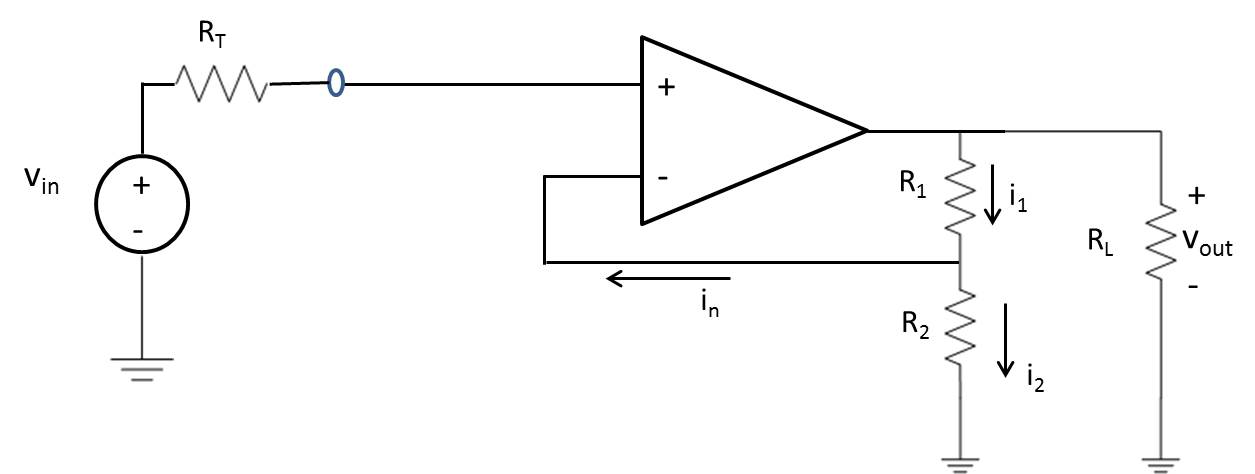
\includegraphics[width=0.7\textwidth]{NonInvertingAmplifier.jpg}
\caption{Non-Inverting Amplifier connected to a Thevenin Circuit}
\label{fig: NonInvertingAmplifier}
\end{figure}

\subsection{Inverting Amplifier}
Figure \ref{fig: InvertingAmplifier} shows an inverting amplifier connected to a thevenin circuit; as mentioned above, this input circuit can represent a non-ideal source or any other resistive circuit.

\begin{figure} [h!]
\centering
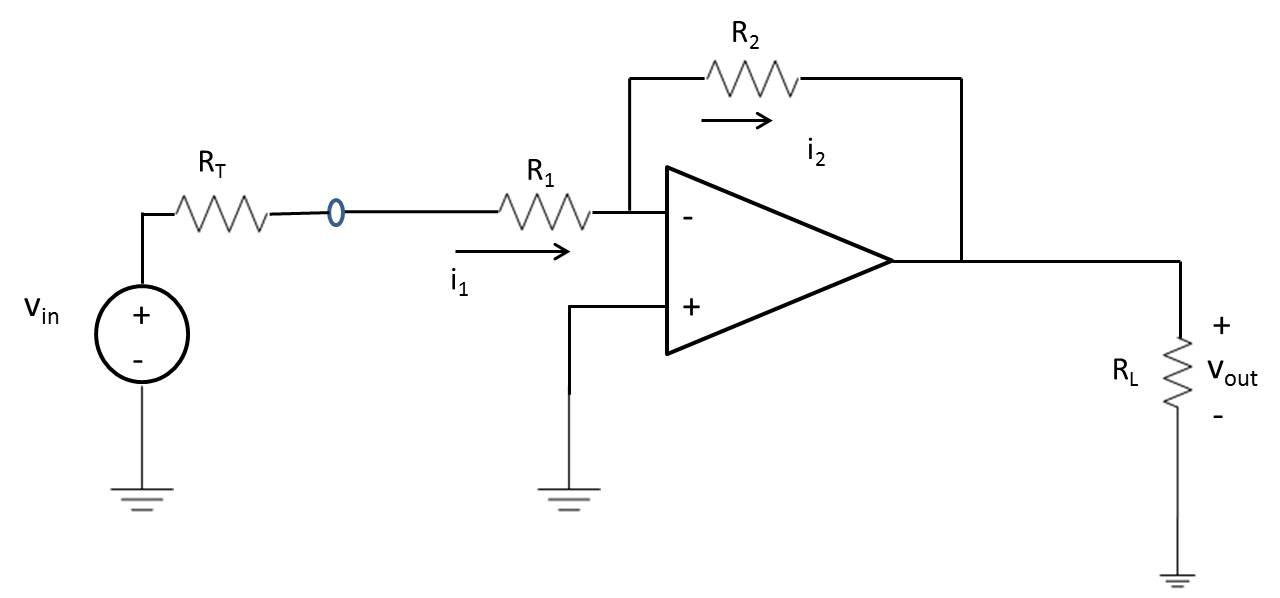
\includegraphics[width=0.7\textwidth]{InvertingAmplifier.jpg}
\caption{Inverting Amplifier connected to a Thevenin Circuit}
\label{fig: InvertingAmplifier}
\end{figure}

In this circuit $R_T$ {\em loads} the input.  This can be thought of a couple of different ways.

\begin{enumerate}
\item $R_T$ is in series with $R_1$.  This will change the transfer characteristic from $K=-\frac{R_2}{R_1}$ to $K=-\frac{R_2}{R_T + R_1}$
\item Since in this circuit current can flow through $R_T$, $V_{in}$ is no longer the input voltage to the Op Amp
\end{enumerate}

\newpage
\clearpage
\pagebreak

\subsection{Summing Amplifier}
Figure \ref{fig: SummingAmplifier} shows a summing amplifier with each input connected to a thevenin circuit; as mentioned above, these input circuits can represent  non-ideal sources or any other resistive circuits.  Using the same logic as for the Inverting Amplifier, it should be obvious that input loading does exist and has to be accounted for.

\begin{figure} [h!]
\centering
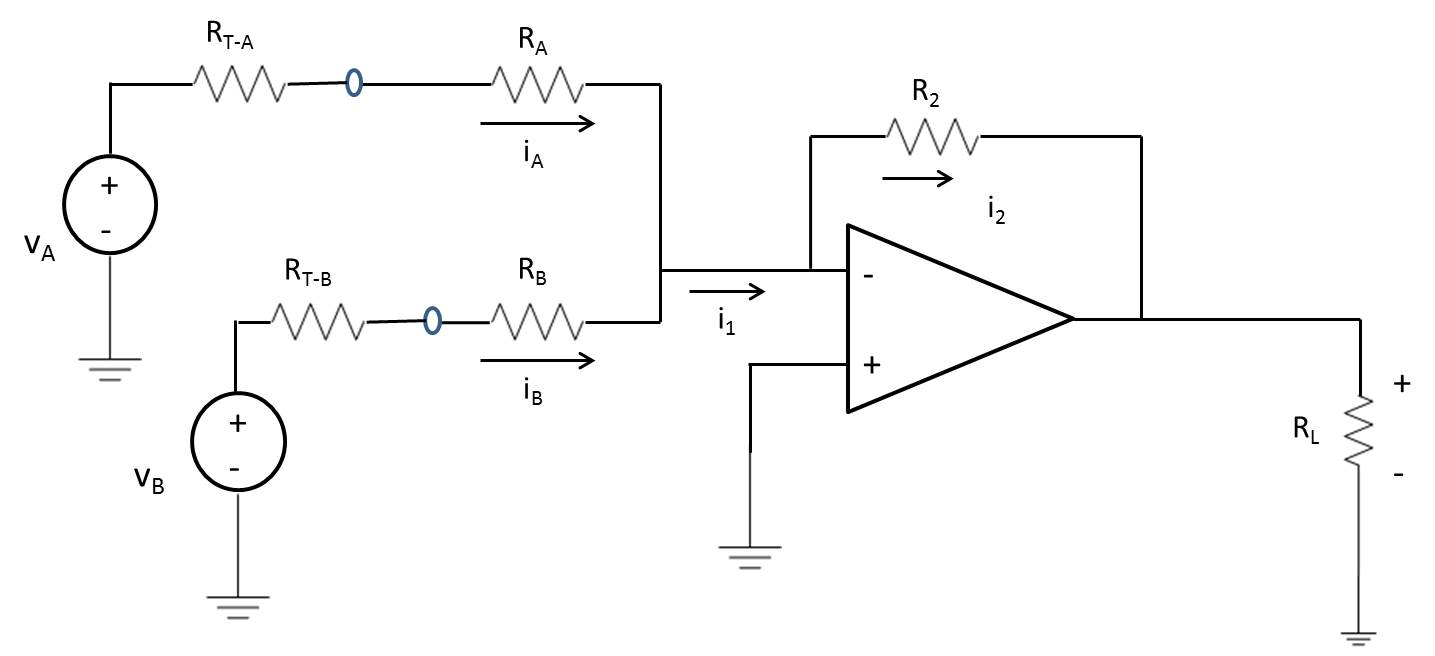
\includegraphics[width=0.6\textwidth]{SummingAmplifier.jpg}
\caption{Summing Amplifier connected to a Thevenin Circuit}
\label{fig: SummingAmplifier}
\end{figure}

\subsection{Differential Amplifier}
Figure \ref{fig: DifferentialAmplifier} shows a differential amplifier with each input connected to a thevenin circuit; as mentioned above, these input circuits can represent  non-ideal sources or any other resistive circuits.  Using the same logic as above, it should be obvious that input loading does exist and has to be accounted for.

\begin{figure} [h!]
\centering
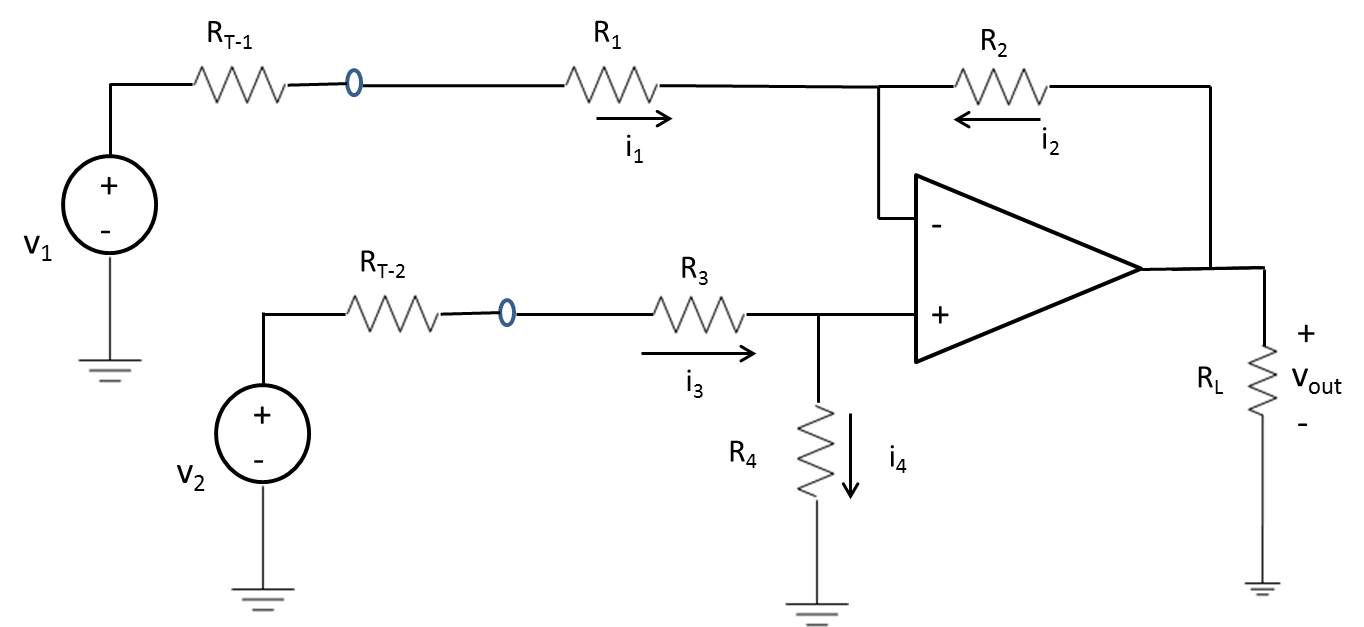
\includegraphics[width=0.6\textwidth]{DifferentialAmplifier.jpg}
\caption{Differential Amplifier connected to a Thevenin Circuit}
\label{fig: DifferentialAmplifier}
\end{figure}

\subsection{Buffer Amplifier}
One way to eliminate input loading is by using a buffer amplifier; see Figure \ref{fig: Buffer}.  It should be obvious that this is a unity gain amplifier and is unaffected by the attached $R_T$.  Placing this circuit before any circuit that is affected by loading will eliminate the effect.

\begin{figure} [h!]
\centering
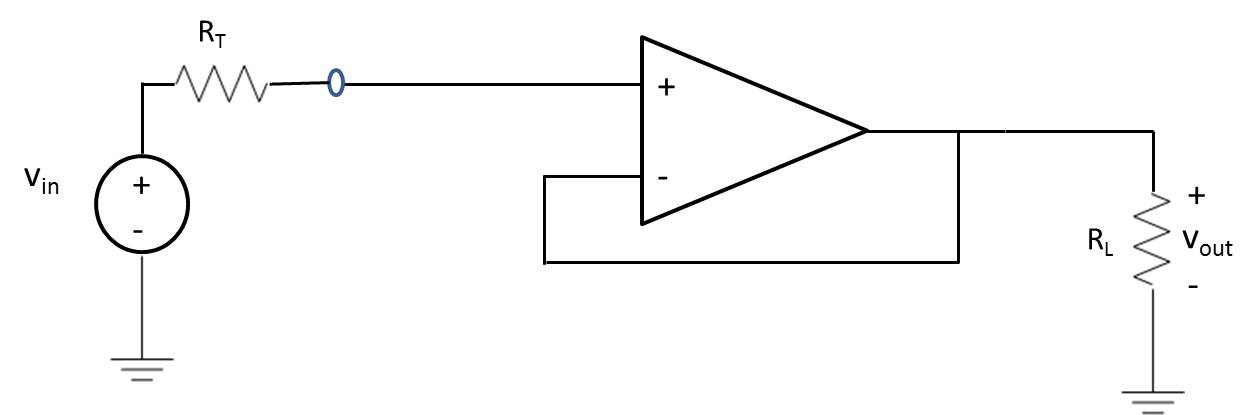
\includegraphics[width=0.6\textwidth]{Buffer.jpg}
\caption{Buffer Amplifier connected to a Thevenin Circuit}
\label{fig: Buffer}
\end{figure}

\newpage
\clearpage
\pagebreak

\section{Op Amp Circuit Design}
This is one of those topics that is best explained just by working examples. Note that because these are design problems, the solutions are not unique; there may be many designs that satisfy the requirements.

\subsection{Example 1 - Cascading}
Design a circuit that gives a gain of 100,000, where the gain of each stage cannot exceed 1,000. Op amps in series are referred to as cascading.

\soln{2.5in}{
To start our design, lets do a quick block diagram:
\begin{figure} [h!]
\centering
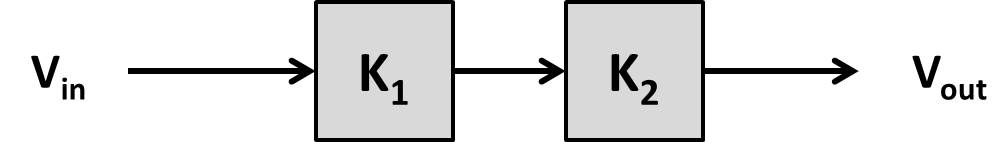
\includegraphics[width=0.6\textwidth]{CascadedGain.jpg}
\end{figure}

The transfer characteristic of this block diagram is
\begin{equation}
V_{out}=K_1K_2V_{in}
\end{equation}
}


Let's look first at a design that cascades two non-inverting amplifiers:

\soln{4.5in}{

\begin{figure} [h!]
\centering
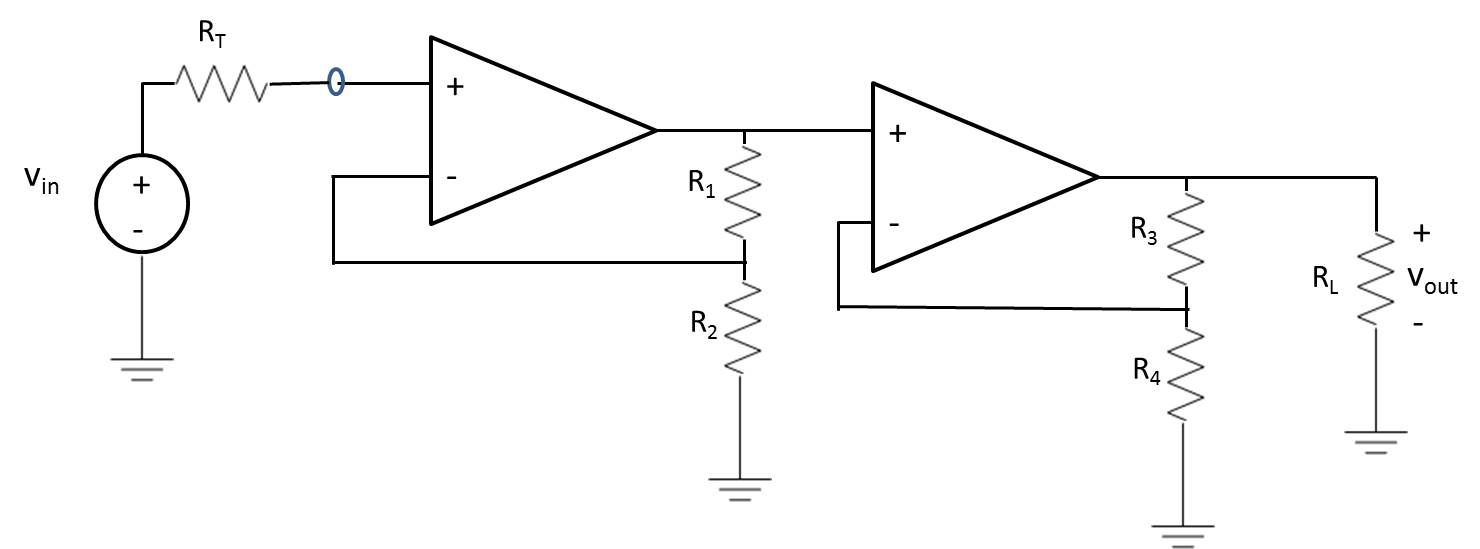
\includegraphics[width=0.7\textwidth]{CascadedNonInvertingAmps.jpg}
\end{figure}

Let's try for a stage 1 gain of $K_1=500$

For stage 1 let's select $R_2 = 1\ k\Omega$ and solve for $R_1$ (recall for a non-inverting amp $K=\frac{R_1+R_2}{R_2}$)
\begin{equation}
R_1 = R_2K_1-R_2 = 1\ k\Omega \times 500 - 1\ k\Omega = 499\ k\Omega
\end{equation}
The closest standard resistance value to $499\ k\Omega$ is $470\ k\Omega$. Resistors are typically available in decade multiples like: 1, 10, 100, 500, 1k, 1.3k, etc. This give an actual gain of
\begin{equation}
K_1=\frac{R_1+R_2}{R_2}=\frac{470\ k\Omega+1\ k\Omega}{1\ k\Omega}=471
\end{equation}
We need a stage 2 gain of $\frac{100,000}{471}=212.3$
Let's use $R_2=2\ k\Omega$ and solve for $R_1$:
\begin{equation}
R_1 = R_2K_1-R_2 = 2\ k\Omega \times 212.3 - 2\ k\Omega = 422.6\ k\Omega
\end{equation}
so we can use an actual value of $R_1 = 430\ k\Omega$ which gives a stage gain of
\begin{equation}
K_2=\frac{R_1+R_2}{R_2}=\frac{430\ k\Omega+2\ k\Omega}{2\ k\Omega}=216
\end{equation}
Total gain is
\begin{equation}
K = K_1K_2 = 417 \times 216 = 101,740
\end{equation}
Because we used non-inverting amplifiers we do not have any loading issues.
}
\newpage
\clearpage
\pagebreak

Let's redo the design with inverting amplifiers:
\soln{6.5in}{
\begin{figure} [h!]
\centering
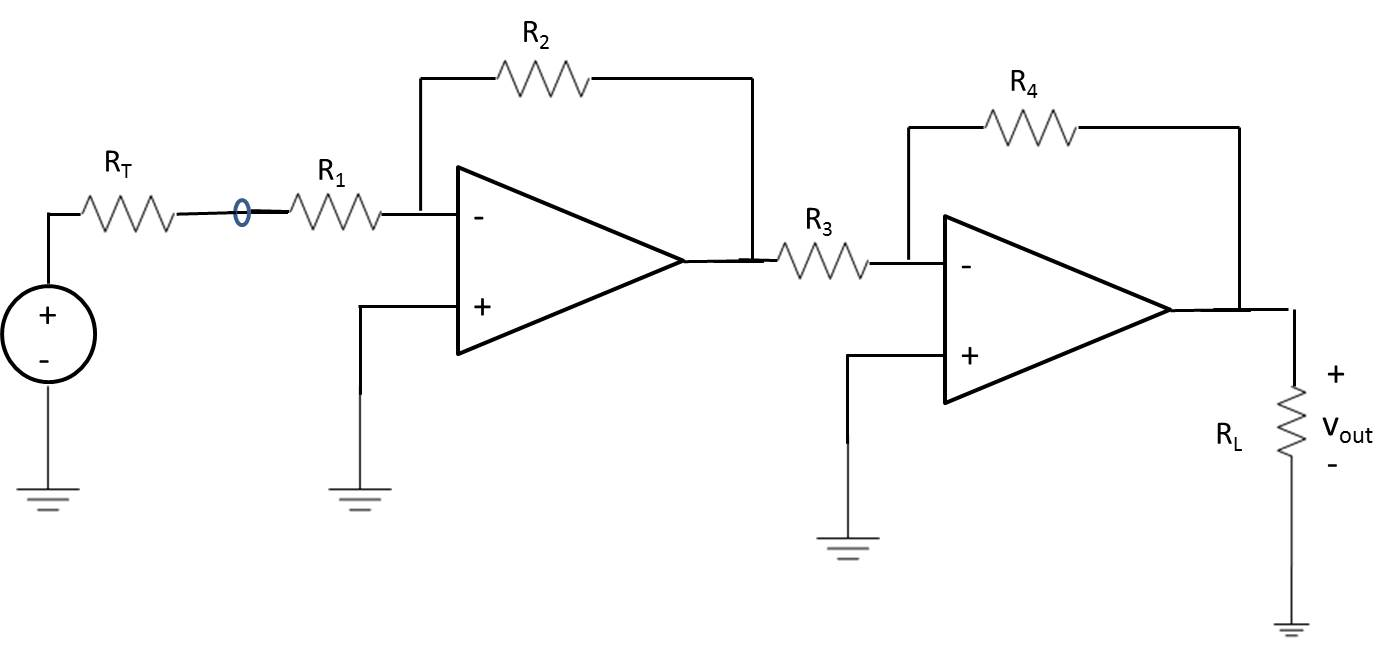
\includegraphics[width=0.7\textwidth]{CascadedInvertingAmps.jpg}
\end{figure}

Since we cascaded two inverting amps we will get a positive overall gain which is what we are after.

But, we have to examine any loading issues.....

What is the gain of the first stage?

\begin{equation}
K_1 = -\frac{R_2}{R_1+R_T}
\end{equation}

It should be already obivious that the resistance of the source is going to affect the gain of the first stage and ultimately the entire system.  Good news is stages do not load each other, so there will be no loading problems on the second stage.

Let's finish the design assuming an $R_T = 100\ \Omega$... Try and get a stage 1 gain of $K_1 = -500$; select $R_1 = 1\ k\Omega$ and solve for $R_2$:
\begin{equation}
R_2 = -K_1(R_1 + R_T) = 500(1\ k\Omega + 100\ \Omega) = 550\ k\Omega
\end{equation}
the closest standard value is $R_2 = 560\ k\Omega$ which gives an actual first stage gain of
\begin{equation}
K_1 = -\frac{560\ k\Omega}{1\ k\Omega + 100\ \Omega}=-509
\end{equation}
so for our second stage we need a gain of $\frac{100,000}{-509}=-196.5$.  Let's use $R_3=1\ k\Omega$ and since there is no stage loading:
\begin{equation}
R_4 = -K_2R_3 = 196.5\times1\ k\Omega = 196.5\ k\Omega
\end{equation}
the closest standard value is $R_4 = 200\ k\Omega$ which gives an actual stage 2 gain of
\begin{equation}
K_2 = -\frac{R_4}{R_3} = -\frac{200\ k\Omega}{1\ k\Omega} = -200
\end{equation}
giving a total gain of
\begin{equation}
K = K_1K_2 = -509 \times -200 = 101,800
\end{equation}
What happens to the total gain if $R_T = 1\ k\Omega$?
Stage one gain changes to
\begin{equation}
K_1 = -\frac{560\ k\Omega}{1\ k\Omega + 1\ k\Omega}=-280
\end{equation}
so total gain is now
\begin{equation}
K = K_1K_2 = -280 \times -200 = 56,000
\end{equation}
}

\newpage
\clearpage
\pagebreak

\textbf{Is there anything we can do to our last design to avoid loading the first stage?}

\soln{4in}{
We can add a buffer amplifier.  Remember a buffer is a unity gain amplifier that does not suffer from stage loading.  The hew design would look like:
\begin{figure} [h!]
\centering
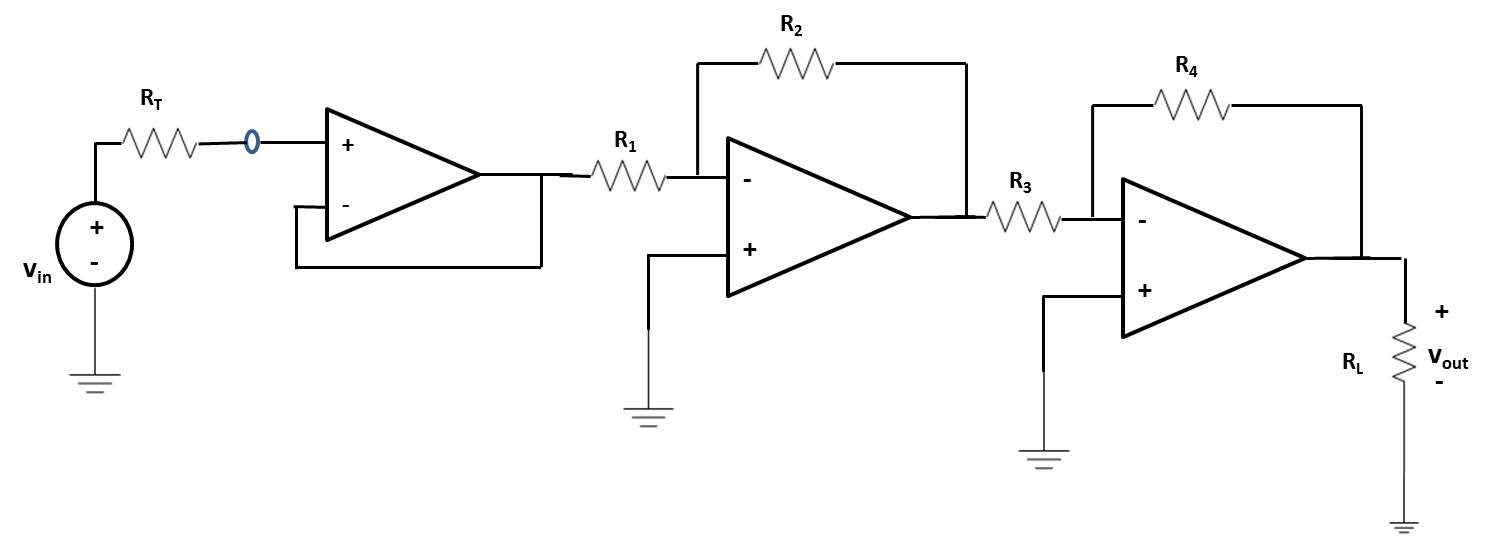
\includegraphics[width=0.7\textwidth]{CascadedInvertingAmpswithBuffer.jpg}
\end{figure}

Since there is no current flowing into the buffer, there is no voltage drop across $R_T$; therefore, there is no loading

}

\subsection{Example 2}
Design an Op Amp circuit that implements the block diagram shown in Figure \ref{fig: Example2}
\begin{figure} [h!]
\centering
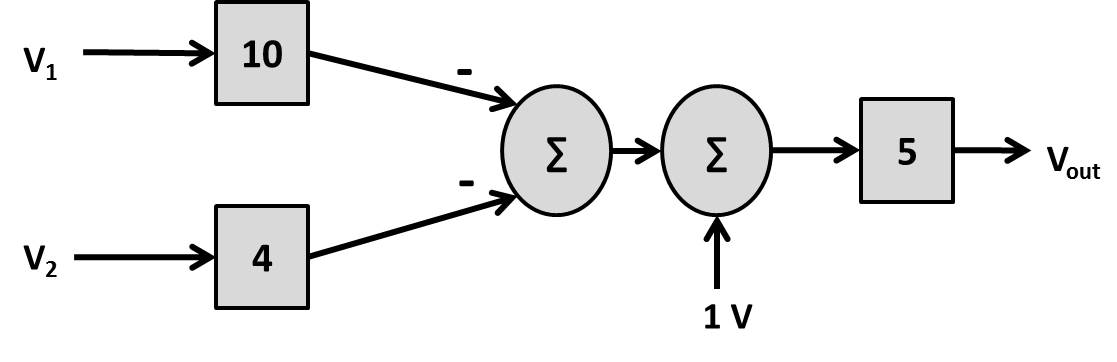
\includegraphics[width=0.5\textwidth]{Example2.jpg}
\caption{Block diagram for example 2}
\label{fig: Example2}
\end{figure}

Designs are not unique.... We will do three designs that work in this example

\soln{3in}{
Start by writing an equation for the transfer characteristic
\begin{equation}
V_{out} = 5(-10V_1-4V_2+1\ V)
\end{equation}
or
\begin{equation}
V_{out} = -50V_1-20V_2+5\ V
\end{equation}
}

\newpage
\clearpage
\pagebreak

For our first design let's build it just like it is drawn with two summers and a final gain stage:

\soln{6in}{
\begin{figure} [h!]
\centering
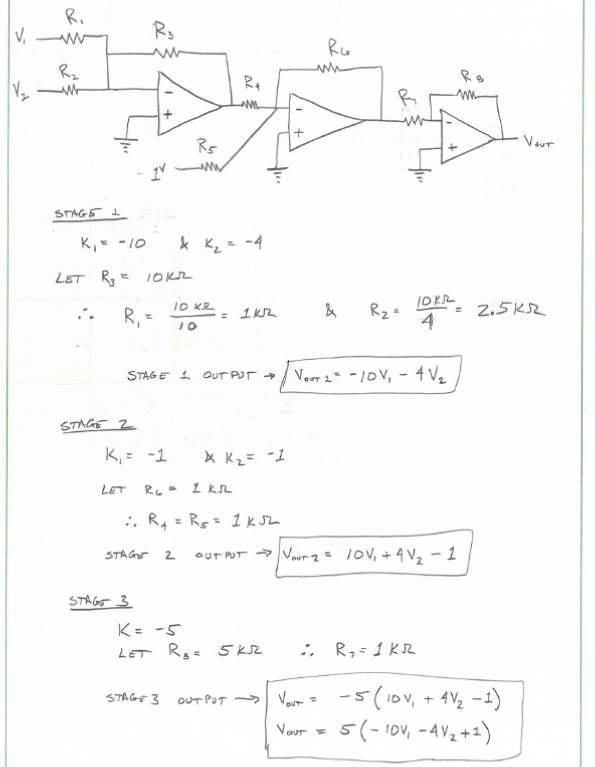
\includegraphics[width=0.9\textwidth]{Example2solnA.jpg}
\end{figure}
This design uses 3 Op Amps and 8 resistors, I think we can be more efficient....
}

\newpage
\clearpage
\pagebreak

Let's combine the summing stages into a single stage; recall we said we can extend the summer design to more than 2 inputs.

\soln{6in}{
\begin{figure} [h!]
\centering
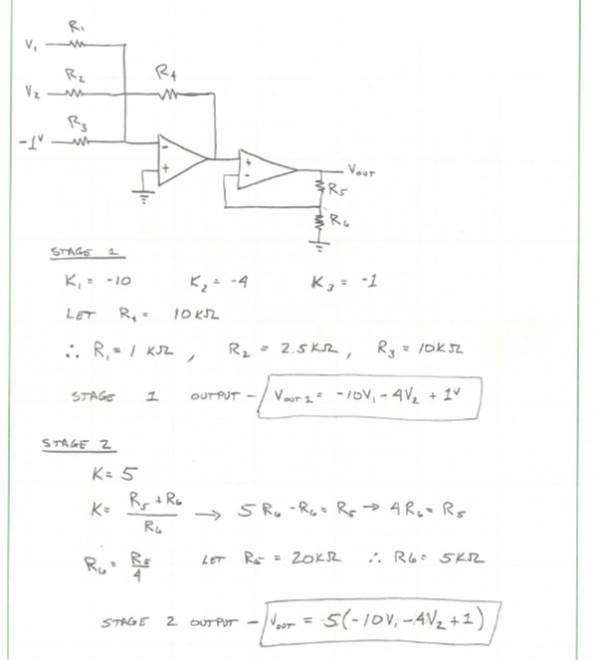
\includegraphics[width=0.9\textwidth]{Example2solnB.jpg}
\end{figure}
This design uses 2 Op Amps and 6 resistors, I still think we can be more efficient....
}

\newpage
\clearpage
\pagebreak

Here is a single stage design that uses 1 Op Amp and 4 resistors

\soln{6in}{
\begin{figure} [h!]
\centering
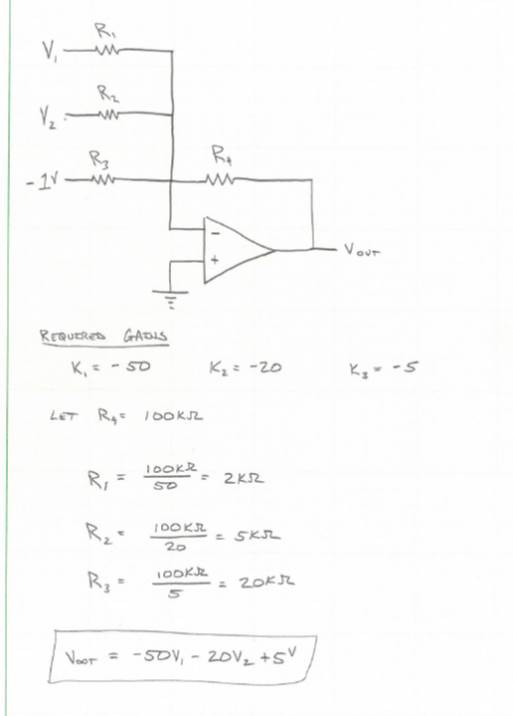
\includegraphics[width=0.9\textwidth]{Example2solnC.jpg}
\end{figure}
}

\newpage
\clearpage
\pagebreak

\newpage
\clearpage
\pagebreak

\newpage
\clearpage
\pagebreak

\newpage
\clearpage
\pagebreak

\newpage
\clearpage
\pagebreak

\end{document}


% Equation Array Example Code
%\begin
%{eqnarray}
%P_R &=& i_R^2R \nonumber \\
%P_R &=& (100\ mA)^2 \times 100\ \Omega \nonumber \\
%P_R &=& (100 \times 10^{-3}\ A)^2 \times 100\ \Omega \\
%P_R &=& 10000 \times 10^{-6}\ A^2  \times 100\ \Omega \nonumber \\
%P_R &=& 1\ W  \nonumber
%\end{eqnarray}

% Figure Example Code
%\begin{figure} [h! t! b!]
%\centering
%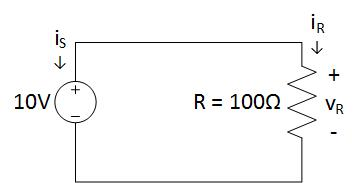
\includegraphics[width=0.5\textwidth]{OhmsLawExampleSolution.jpg}
%\caption{Ohm's Law example circuit}
%\label{fig: OhmsLawExampleSolution}
%\end{figure}

%Table Example Code
%\begin{table}[h]
%\centering
%\begin{tabular}{|l|c|c|}
%\hline
%Prefix & Abbreviation & Value \\
%\hline \hline
%Giga & $G$ & $10^9$ \\
%Mega & $M$ & $10^6$ \\
%Kilo & $k$ & $10^3$ \\
%\hline
%milli & $m$ & $10^{-3}$ \\
%micro & $\mu$ & $10^{-6}$ \\
%nano & $n$ & $10^{-9}$ \\
%pico & $p$ & $10^{-12}$ \\
%\hline
%\end{tabular}
%\caption{Engineering prefixes and values}
%\label{tab: Eng Prefixes}
%\end{table}
